\documentclass[tikz,border=8pt]{standalone}
\usepackage[T1]{fontenc}
\usepackage{times}
\usetikzlibrary{arrows.meta,positioning}
\begin{document}
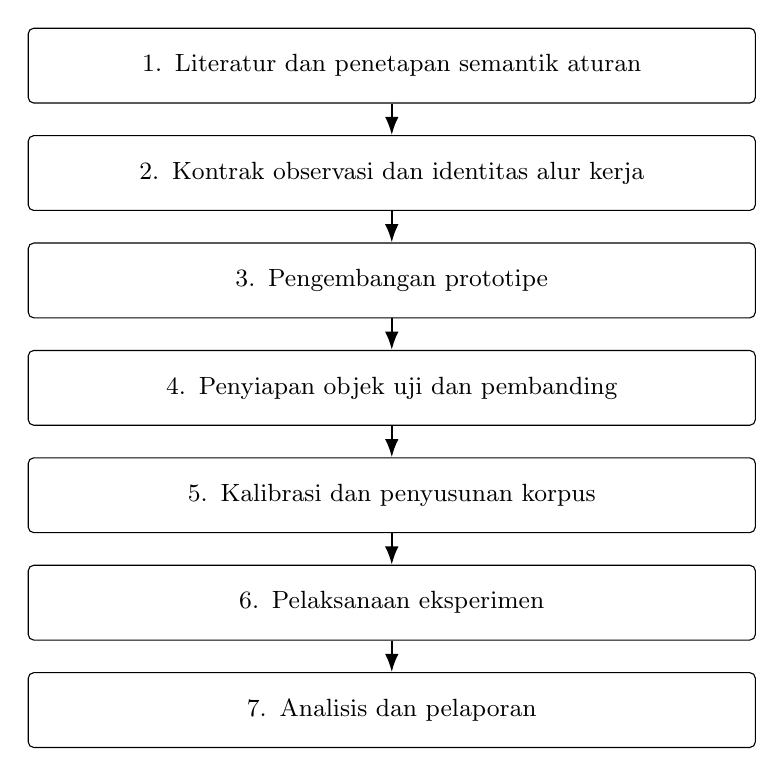
\begin{tikzpicture}[box/.style={draw,rounded corners=2pt,align=center,
  text width=9cm,minimum height=0.95cm,font=\small},
  arrow/.style={-{Latex},thick},node distance=0.4cm]
  \node[box] (a) {1. Literatur dan penetapan semantik aturan};
  \node[box,below=of a] (b) {2. Kontrak observasi dan identitas alur kerja};
  \node[box,below=of b] (c) {3. Pengembangan prototipe};
  \node[box,below=of c] (d) {4. Penyiapan objek uji dan pembanding};
  \node[box,below=of d] (e) {5. Kalibrasi dan penyusunan korpus};
  \node[box,below=of e] (f) {6. Pelaksanaan eksperimen};
  \node[box,below=of f] (g) {7. Analisis dan pelaporan};
  \draw[arrow] (a) -- (b); \draw[arrow] (b) -- (c);
  \draw[arrow] (c) -- (d); \draw[arrow] (d) -- (e);
  \draw[arrow] (e) -- (f); \draw[arrow] (f) -- (g);
\end{tikzpicture}
\end{document}
